%导言区,笔记模板
\documentclass{article}

\usepackage{ctex}
\title{机器学习笔记}
\author{cuihu}
\date{\today}

\usepackage[a4paper,left=10mm,right=10mm,top=15mm,bottom=15mm]{geometry} 
\usepackage{listings}
\setlength{\parindent}{0pt}% 去掉首行缩进。

\usepackage{titlesec}%设置标题格式。/
%\titleformat{\section}{\centering}
%\titleformat{\section}{\centering\Huge\bfseries}{第\,\thechapter\,章}{1em}{}
%\titleformat{\section}{\lef}{label}{sep}{before-code}[after-code]

\usepackage{graphicx}
\usepackage{hyperref}
%\usepackage{hyperref}/



\begin{document}
	\maketitle
	\begin{abstract}
		菜菜sklearn 笔记	
	\end{abstract}

\section{PCA与SVD降维算法}
		我们希望能够找出一种办法来帮助
		我们衡量特征上所带的信息量,让我们在降维的过程中,\emph{能够即减少特征的数量,又保留大部分有效信息}——将那
		些带有重复信息的特征合并,并删除那些带无效信息的特征等等——逐渐创造出能够代表原特征矩阵大部分信息
		的,特征更少的,新特征矩阵。
		
		
	   从方差的这种应用就可以推断出,如果一个特征的方差很大,则说
	   明这个特征上带有大量的信息。因此,在降维中,{\heiti 使用的信息量衡量指标,就是样本方差,又称可解释性方差,方差越大,特征所带的信息量越多。}
	 
		$$V a r=\frac{1}{n-1} \sum_{i=1}^{n}\left(x_{i}-\hat{x}\right)^{2}$$
		
		Var代表一个特征的方差,n代表样本量,xi代表一个特征中的每个样本取值,xhat代表这一列样本的均值。
	
	\subsection{实现}
	
	\begin{lstlisting}[language=python]
		class  sklearn.decomposition.PCA (
		n_components=None, 
		copy=True, 
		whiten=False, 
		svd_solver=’auto’, 
		tol=0.0,
		iterated_power=’auto’, 
		random_state=None)
	\end{lstlisting}
	
	\begin{figure}[htpb]
		\centering
		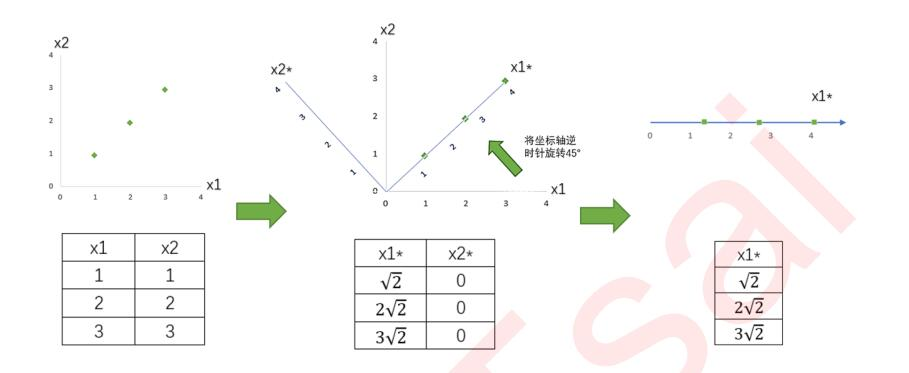
\includegraphics[width=\linewidth]{skl_fig/sk1}
		\caption{二维降一维}
	\end{figure}
	{\heiti 找出n个新特征向量,让数据能够被压缩到少数特征上并且总信息量不损失太多的技术就是
	矩阵分解。}
	
	
	PCA使用方差作为信息量的衡量指标,并且特征值分解来找出空间V。降
	维时,它会通过一系列数学的神秘操作(比如说,产生协方差矩阵 )将特征矩阵X分解为以下三个矩阵,其
	中 和 是辅助的矩阵,Σ是一个对角矩阵(即除了对角线上有值,其他位置都是0的矩阵),其对角线上的元素
	就是方差。降维完成之后,PCA找到的每个新特征向量就叫做“主成分”,而被丢弃的特征向量被认为信息量很少,
	这些信息很可能就是噪音。
	
	\begin{equation}
		X  \rightarrow Q \Sigma Q^{-1}
	\end{equation}
	
	而SVD使用奇异值分解来找出空间V,其中Σ也是一个对角矩阵,不过它对角线上的元素是奇异值,这也是SVD中用
	来衡量特征上的信息量的指标\verb|。U和V^{T}|分别是左奇异矩阵和右奇异矩阵,也都是辅助矩阵。
	
	$$ X  \rightarrow U \Sigma V^{T} $$
	
	\subsection{思考:PCA和特征选择技术都是特征工程的一部分,它们有什么不同?}
	特征工程中有三种方式:特征提取,特征创造和特征选择。仔细观察上面的降维例子和上周我们讲解过的特征
	选择,你发现有什么不同了吗?\\
	特征选择是从已存在的特征中选取携带信息最多的,选完之后的特征依然具有可解释性,我们依然知道这个特
	征在原数据的哪个位置,代表着原数据上的什么含义。\\
	而PCA,是将已存在的特征进行压缩,降维完毕后的特征不是原本的特征矩阵中的任何一个特征,而是通过某
	些方式组合起来的新特征。通常来说,在新的特征矩阵生成之前,我们无法知晓PCA都建立了怎样的新特征向
	量,新特征矩阵生成之后也不具有可读性,我们无法判断新特征矩阵的特征是从原数据中的什么特征组合而
	来,新特征虽然带有原始数据的信息,却已经不是原数据上代表着的含义了。{\heiti 以PCA为代表的降维算法因此是
	特征创造(feature creation,或feature construction)的一种。}\\
	可以想见,PCA一般不适用于探索特征和标签之间的关系的模型(如线性回归),因为无法解释的新特征和标
	签之间的关系不具有意义。在线性回归模型中,我们使用特征选择。\\
	
	\subsection{参数}
	\begin{lstlisting}[language=python]
	class  sklearn.decomposition.PCA (
	n_components=None, 
	copy=True, 
	whiten=False, 
	svd_solver=’auto’, 
	tol=0.0,
	iterated_power=’auto’, 
	random_state=None)
	\end{lstlisting}
	
	\subsubsection{重要参数n\_components}
	该参数就是我们需要降维的目标个数,如果我们需要可视化一组特征,那么降低到二维,以下就是例子。
	:
	\hrule
	
	\begin{lstlisting}[language=python]
	# 调用模块
	import matplotlib.pyplot as plt
	from sklearn.datasets import load_iris # 数据集。
	from sklearn.decomposition import PCA # PCA
	
	# 提取数据集
	import matplotlib.pyplot as plt
	from sklearn.datasets import load_iris
	from sklearn.decomposition import PCA
	
	# 提取数据集。
	iris = load_iris()
	y = iris.target
	x = iris.data
	
	
	
	# 作为数据表或特征矩阵,x 是几维度。
	
	print(x.shape)
	
	import pandas as pd
	df = pd.DataFrame(x)   #(150,4)
	# print(df)# 可以看出一共有四个特征,150行。
	
	# 建模
	pca = PCA(n_components=2)
	# 实例化。
	pca = pca.fit(X=x)
	x_dr = pca.transform(x)
	print(x_dr.shape) # 从思维转换到了二维。 (150,2)
	
	# 可视化。
	x_dr[y == 0, 0]
	# 第一种话花的索引。
	# 标签的为 0 1 2
	# plt.figure()
	# plt.scatter(x_dr[y==0, 0], x_dr[y==0, 1], c="red", label=iris.target_names[0])
	# plt.scatter(x_dr[y==1, 0], x_dr[y==1, 1], c="black", label=iris.target_names[1])
	# plt.scatter(x_dr[y==2, 0], x_dr[y==2, 1], c="orange", label=iris.target_names[2])
	# plt.legend()
	# plt.title('PCA of IRIS dataset')
	# plt.show()
	
	colors = ['red', 'black', 'orange']
	iris.target_names
	plt.figure()
	for i in [0, 1, 2]:
	plt.scatter(x_dr[y == i, 0],
	x_dr[y == i, 1],
	alpha=.7,
	c=colors[i],
	label=iris.target_names[i])
	plt.legend()
	plt.title('PCA of IRIS dataset')
	plt.show()
	
	
	#探索降维后的数据
	# 属性explained_variance_, 查看降维后每个特征向量上所带的信息量大小。(可解释方差大小)
	print(pca.explained_variance_)  # 可解释方差大小。
	
	# 可解释方差贡献率。也就是新的特征向量对原始特征的信息量的贡献率。 [4.22824171 0.24267075]
	print(pca.explained_variance_ratio_)   # [0.92461872 0.05306648]
	
	# 大部分信息被集中在了第一维。
	
	print(pca.explained_variance_ratio_.sum())  #0.9776852063187951
	
	# 选择最好的n_components:累积可解释方差贡献率曲线
	
	
		
		
	\end{lstlisting}
	
	\subsubsection{选择最好的n\_components:累计可解释方差贡献率曲线}
	当参数n\_components中不填写任何值,则默认返回min(X.shape)个特征,一般来说,样本量都会大于特征数目,
	所以什么都不填就相当于转换了新特征空间,但没有减少特征的个数。一般来说,不会使用这种输入方式。但我们
	却可以使用这种输入方式来画出累计可解释方差贡献率曲线,以此选择最好的n\_components的整数取值。\\
	累积可解释方差贡献率曲线是一条以降维后保留的特征个数为横坐标,降维后新特征矩阵捕捉到的可解释方差贡献
	率为纵坐标的曲线,能够帮助我们决定n\_components最好的取值。
	
	\begin{lstlisting}[language = python]
		import numpy as np
		pca_line = PCA().fit(x)  #没有参数。
		plt.plot([1,2,3,4], np.cumsum(pca_line.explained_variance_ratio_))
		plt.xticks([1,2,3,4])
		plt.grid()
		plt.xlabel('number of components after dimension reduction')
		plt.ylabel('cumulative explained variance ratio')
		plt.show()
	\end{lstlisting}
	
	\subsubsection{最大似然估计选择超参数}
	
	除了输入整数,n\_components还有哪些选择呢?之前我们提到过,矩阵分解的理论发展在业界独树一帜,勤奋智
	慧的数学大神Minka, T.P.在麻省理工学院媒体实验室做研究时找出了让PCA用最大似然估计(maximum likelihood
	estimation)自选超参数的方法,输入“mle”作为n\_components的参数输入,就可以调用这种方法。
	
	\begin{lstlisting}[language = python]
		pca_mle = PCA(n_components='mle')
		pca_mle = pca_mle.fit(x)
		x_mle = pca_mle.transform(x)
		
		print(x_mle.shape)  # (150, 3)
		
		print(pca_mle.explained_variance_ratio_.sum())  # 0.9947878161267248
	\end{lstlisting}
	
	
	\subsubsection{按信息量占比选超参数}
	
	输入[0,1]之间的浮点数,并且让参数svd\_solver =='full',表示希望降维后的总解释性方差占比大于n\_components
	指定的百分比,即是说,希望保留百分之多少的信息量。比如说,如果我们希望保留97\%的信息量,就可以输入
	n\_components = 0.97,PCA会自动选出能够让保留的信息量超过97\%的特征数量。
	
	\begin{lstlisting}[language = python]
		pca_f = PCA(n_components=0.97, svd_solver='full').fit(x)  # 大于百分之97即可。
		x_f = pca_f.transform(x)
		print(pca_f.explained_variance_ratio_)
		print(x_f.shape)
	\end{lstlisting}
	
	\subsection{PCA中的SVD}
	\subsubsection{PCA中的SVD哪里来?}
	
	
\end{document}
